\section{Connessione}
Un grafo si dice \textit{connesso} se - a partire da un nodo qualsiasi - posso raggiungerne un altro qualsiasi.
Qualora non sia connesso, si definisce \textit{componente connesso} qualsiasi sezione connessa che lo compone.

\section{Visitare un grafo}
Esistono due tipi di visita:
\begin{enumerate}
    \item Visita in profondità
    \item Visita in ampiezza
\end{enumerate}

\subsection{Visita in profondità}
Rappresenta una visita ricorsiva del grafo, partendo da un nodo generico scelto arbitrariamente. \\
Si costruisce un vettore binario \textit{v} (i cui valori sono inizialmente impostati tutti a \textit{0} - con costo $O(n)$), composto da n componenti, utilizzato per tenere traccia se il nodo preso in esame è già stato visitato (e quindi il suo valore sul vettore sarà impostato ad \textit{1}) o meno.\\
\begin{center}
    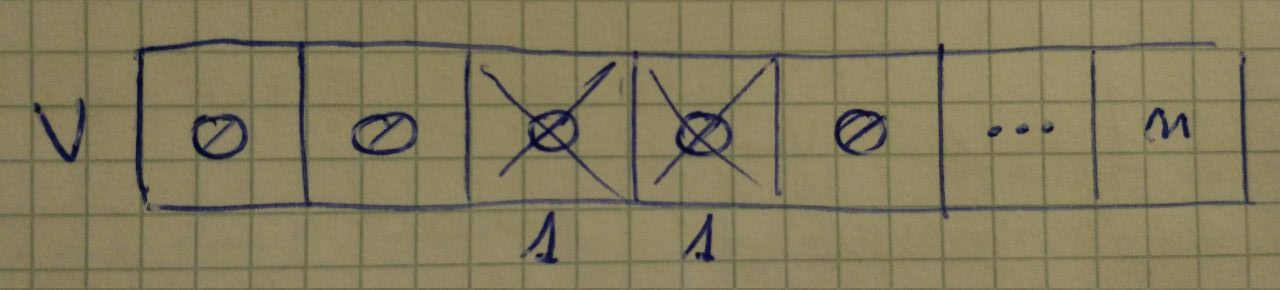
\includegraphics[width=.8\textwidth]{vettore-visita.jpg} \hfill
\end{center}
\newpage

Inizializzato il vettore a \textit{0}, eseguo la procedura \textit{DFS(x)}:
\begin{lstlisting}
DFS(x)
    vis[x] <- 1         # imposto il valore del nodo ad 1
    for y in adj(x)     # itero sui nodi adiacenti ad x
        if vis[y]==0 then DFS(y)
\end{lstlisting}

Chiaramente, se al termina della visita, \textit{v} contiene ancora alcuni \textit{0}, significa che il grafo non è connesso. \\
Genericamente la procedura \textit{DFS(x)} ha complessità di $O(n)$. Inoltre, però, questa fa un'iterazione (attraverso il ciclo \textit{for}) per ogni adiacenza col nodo, impiegando - nel caso peggiore - \textit{n} - caso in cui, quindi, il nodo abbia numero di adiacenze pari al numero totale di nodi. Di conseguenza, la procedura di visita impiega al più $O(n^2)$. \\
Se questa procedura - invece di lavorare con un vettore - lavora sulla rappresentazione a matrice, il caso peggiore che abbiamo analizzato, diventa l'unico caso possibile, per cui $\theta(n^2)$. \\
Infine, utilizzando la rappresentazione tramite liste di adiacenze, la procedura avrà complessità $O(n+m)$. \\\\
Tramite il percorso seguito dalle chiamate \textit{DFS(x)} è inoltre possibile ricavarci un albero, la cui radice è proprio la sorgente da cui si è partiti nella visita del grafo. \\
Inoltre, tramite lo stesso algoritmo - aggiungendo codice e/o funzioni - è possibile ottenere funzionalità particolari e aggiuntive, come la costruzione di un \textit{vettore dei padri}, un vettore che associa ad ogni nodo il corrispettivo padre nella rappresentazione dell'albero ottenuto tramite la visita del grafo.